\section{Introduction}
\label{sec:introduction}

With the end of Dennard Scaling~\cite{dennard}, the amount of performance one can extract from a CPU is reaching a limit.
To provide general-purpose flexibility, CPU spends the majority of energy on overheads, including dynamic-instruction execution, branch prediction, and a cache hierarchy, and less than 20\% of the energy on the actual computation~\cite{mark}.
Even worse, the power wall is limiting the entire multicore family
to reach the doubled performance improvement per generation enabled by technology scaling in the past\cite{multicorescale}.

For this reason, many recent efforts are spent on leveraging application domain knowledge in hardware design to enable 
continued performance scaling while meeting the power budget\cite{turinglecture}.
Examples include widely adopted General-Purpose Graphics Processing Units (GPGPUs) in the deep-learning domain and machine learning (ML) accelerators, such as Tensor Processing Units~\cite{tpu} and EIE~\cite{eie}, providing orders of magnitude acceleration over a CPU.
However, massive threads in GPU and the highly specialized datapath in ML accelerators often cause severe
underutilization of the hardware due to variation in application and data characteristics\cite{tz_rnn}.

\begin{figure}[!tbp]
  \centering
  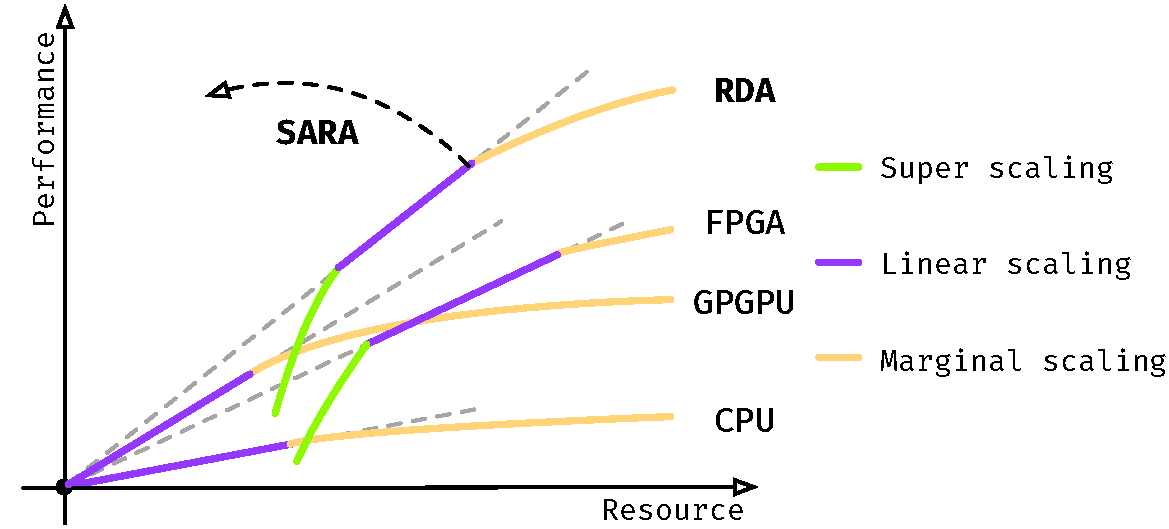
\includegraphics[height=0.1\paperheight]{figures/parpipe.pdf}
  \caption{Scaling regimes for processor (CPU and GPGPU) and spatial architectures (FPGA and RDA).}
  \label{fig:scaling}
  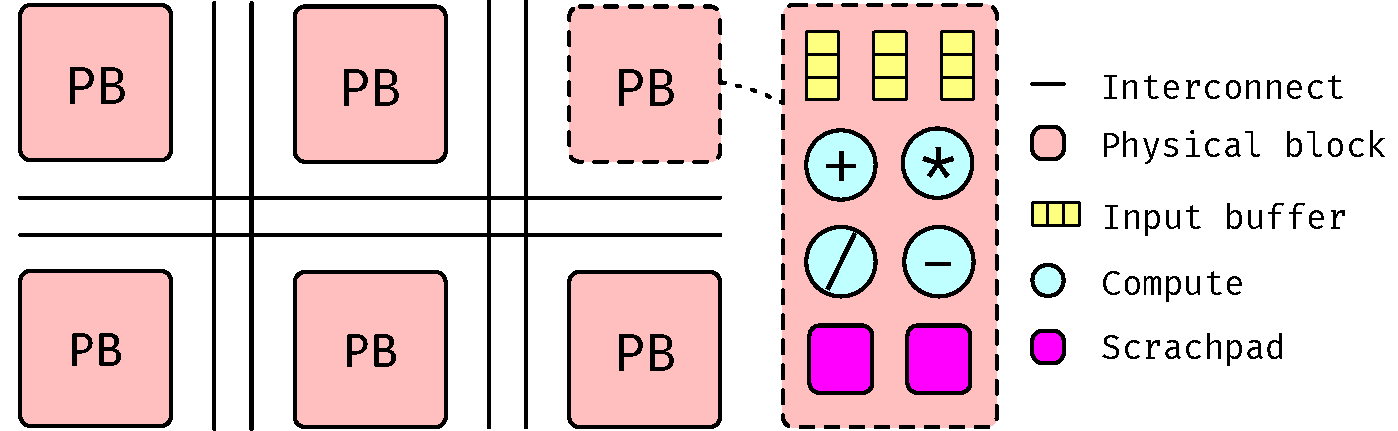
\includegraphics[width=1\columnwidth, height=0.1\paperheight, keepaspectratio]{figures/rda_arch.pdf}
  \caption{RDA High-Level Model}\label{fig:arch}
\end{figure}

Reconfigurable spatial architectures overcome this limitation by changing its datapath based on applications' needs.
Applications are configured at the circuit-level without dynamic instruction fetching and decoding, hence improving energy-efficiency.
In addition to instruction, data, and task-level parallelism explored by processor architectures, spatial architectures also explore instruction and task-level
pipelining that further increase the compute throughput.
Pipelining at various granularity enables spatial architectures to achieve high throughput on program phases without massive parallel workload, and allocate resource proportional to compute intensities of program phases.
As the whole program is pipelined, performance is bounded by the bottleneck stage with the highest latency.
Initially, the overall throughput can be doubled by only parallelizing the bottleneck stage without doubling the resource of the entire program, which gives a super scaling in performance to allocated resources, shown in \Cref{fig:scaling}.
After stage-balancing, programs enter the linear scaling regime with proportional performance to resource increase, similar
to the best achievable scaling on processor architectures.
Eventually, communication overheads cause sub-linearly scaling in all architectures.
Many applications inherently contain imbalanced workloads in their program structures. 
For example, layers of a deep neural network vary highly in operational complexity.
Spatial architectures can take advantage of imbalance workloads in a program to achieve
high marginal performance improvement per resource increase in the super scaling regime.
For applications, such as large image network like ResNet\cite{resnet}, RDAs tend to run out of resource before
balancing the pipeline, which leaves the program entirely in the super scaling regime.

One example of a spatial architecture is Field Programmable Gate Arrays (FPGAs) that support fine-grain, 
bit-level reconfiguration with a soft logic fabric~\cite{fpga-survey}.
Although around for a long time, FPGAs are not broadly used on high-level applications due to their low-level programming interface 
and low resource density with high routing overhead.

Lately, Reconfigurable Dataflow Accelerators (RDAs)~\cite{plasticine, ti} are emerging as a new class of spatial accelerators that retain the desired level of flexibility and energy efficiency without the fine-grained reconfigurability overhead.
RDA provides high resource density and compute throughput with a hierarchical streaming network, operating at a fixed and high clock frequency at large chip sizes.
Recent studies~\cite{plasticine} have demonstrated a promising acceleration of dense, sparse, and streaming applications using RDAs.

Today, these RDAs are controlled using centralized-control schemes to manage and schedule the spatially distributed compute and memory resources.
However, to accommodate applications with ever-increasing sizes (\eg, large deep neural networks), architects are building ever-larger RDAs.
At scale, the centralized schemes incur high synchronization overhead and communication hot spots. 
To achieve complex control schemes, such as a while convergence, a host often has to launch the RDA multiple times and materialize the on-chip states to DRAM, which further degrades performance.
Moreover, as RDAs become larger, their coarse-grained hierarchal structure introduces fragmentation in resource allocation.
Traditional mapping strategies---performing one-to-one allocation of resource tiles to program constructs---results in severe underutilization of resources, and heterogeneity in RDA resources further decreases mapping efficiency.

In this paper, we introduce \name{}---a compiler for scaling performance and enhancing mapping efficiency for RDAs. 
We propose a distributed p2p control paradigm that minimizes synchronization overhead for RDAs at scale.
We show that \name{} can infer synchronization required for on-chip distributed execution from an application, written in a sequential, unpipelined programming abstraction.
We present a mapping strategy efficiently decomposing a program over the distributed collection of compute and memory resources with global optimizations, which significantly reduces resource fragmentation for RDAs with heterogeneous resources (\Cref{sec:background}).
The distributed control improves RDA's performance by extending the linear region in the performance-resource curve in \Cref{fig:scaling}.
Whereas, the mapping strategy and optimizations reduce the fragmentation and, hence, pushes the scaling curve left.

Using a recently published RDA--Plasticine~\cite{plasticine}--as the target architecture, our evaluation shows that \name improves Plasticine's scaling efficiency (\Cref{ssec:scalability})\yz{quantify this}.
We qualitatively evaluate the impacts of individual optimizations on performance and resource (\Cref{ssec:evalopts}), and compare to a state-of-art Tesla V100 GPU (\Cref{ssec:abs-performance}).
We begin with a brief background on RDA architecture and the input of \name{} (\Cref{sec:background}), before detailing the design of our compiler (\Cref{sec:compiler}). 
